% !TEX program = xelatex
\documentclass[12pt,a4paper]{article}
\usepackage[T1]{fontenc}
%\usepackage{tgpagella, eulervm}

% --- XeLatex/LuaLatex --- 
\usepackage[no-math]{fontspec}
\IfFontExistsTF{Fira Sans}{
	\setmainfont{Fira Sans}
}

% % --- This is for pdflatex ---
%\usepackage[light, sfdefault]{FiraSans}

\usepackage[italic]{mathastext}
\usepackage[bahasa]{babel}
\usepackage{booktabs}
\usepackage{geometry}
\usepackage{tabularx}
\usepackage{graphicx}
\usepackage{float}
\usepackage{xcolor}
\usepackage{hyperref}
\hypersetup{
	colorlinks=true,  % Colours links instead of boxes
	urlcolor=blue,    % Colour for external hyperlinks
	linkcolor=blue,   % Colour of internal links (sections, etc.)
	citecolor=red,    % Colour of citations
	bookmarks=true,   % Adds PDF bookmarks
	hypertexnames=true
}

\geometry{left=2cm, right=2cm, top=2cm}
\title{\textbf{Panduan Menghitung \textit{Signal--to--Noise Ratio} (SNR)} dengan AstroImageJ (AIJ)}
\author{Observatorium Bosscha}
\hyphenation{me-la-ku-kan peng-amat-an deng-an}
\begin{document}
\maketitle
\noindent\rule{\linewidth}{0.4pt}

\textit{Signal--to--Noise Ratio} (SNR) adalah ukuran kualitas data yang menyatakan seberapa besar sinyal yang diukur dibandingkan dengan tingkat kebisingan dalam data tersebut. Secara umum, SNR dinyatakan dalam persamaan berikut
\begin{equation}
	SNR = \frac{Signal}{Noise}
\end{equation}

Dalam konteks CCD/CMOS, SNR dirumuskan sebagai berikut
\begin{equation}
	SNR = \frac{S}{\sqrt{S + n_{pix} (B + RN^2)}}
\end{equation}
di mana $S$ adalah jumlah total sinyal (dalam satuan elektron) yang diterima dari sumber, $n_{pix}$ adalah jumlah piksel yang digunakan untuk mengukur sinyal, $B$ adalah jumlah rata--rata elektron latar belakang per piksel, dan $RN$ adalah \textit{noise} pembacaan per piksel (dalam satuan elektron).
Persamaan di atas adalah model praktis untuk estimasi awal SNR. Pada kondisi sebenarnya, nilai SNR juga dipengaruhi oleh kualitas kalibrasi (bias/dark/flat), kestabilan langit, fokus, serta akurasi pemilihan aperture dan annulus latar belakang.

Panduan berikut akan menunjukkan cara menghitung SNR menggunakan \textit{software} AstroImageJ (AIJ) dengan data yang diambil menggunakan \textsc{SharpCap}. Pastikan Anda sudah memiliki data yang siap untuk dianalisis, dan ikuti langkah--langkah berikut untuk mendapatkan nilai SNR dari data Anda.

\begin{enumerate}
	\item Download AIJ dari tautan berikut (\url{https://astroimagej.com/downloads/}). Sesuaikan dengan sistem operasi yang digunakan.
	\item Lakukan instalasi seperti biasa, semua pilihan dalam keadaan \textit{default}.
	\item Siapkan folder kerja yang berisi file--file yang akan dicari SNR--nya. Pada contoh ini hanya digunakan 5 file saja tanpa file kalibrator (bias, dark, flat). Pastikan nama file memiliki pola tertentu, misal \textbf{namatarget\_exptime}. Secara default \textsc{SharpCap} akan memberikan penamaan file secara urut.
	\begin{center}
		\includegraphics[width=0.6\linewidth]{snr_data_folder}
	\end{center}
	
	\item Buka \textsc{AIJ}, maka akan muncul tampilan berikut.
	\begin{center}
		\includegraphics[width=0.6\linewidth]{snr_aij}
	\end{center}
	
	\item Pilih \textit{File > Import > Image Sequence}, maka akan muncul tampilan berikut. Pastikan centang `Use virtual stack'.
	
	\underline{Catatan:} tampilan frame berikut berada dalam mode \textit{invert}. Tekan logo dalam kotak merah untuk \textit{toggle}.
	\begin{center}
		\includegraphics[width=0.6\linewidth]{snr_aij_import}
	\end{center}
	\begin{center}
		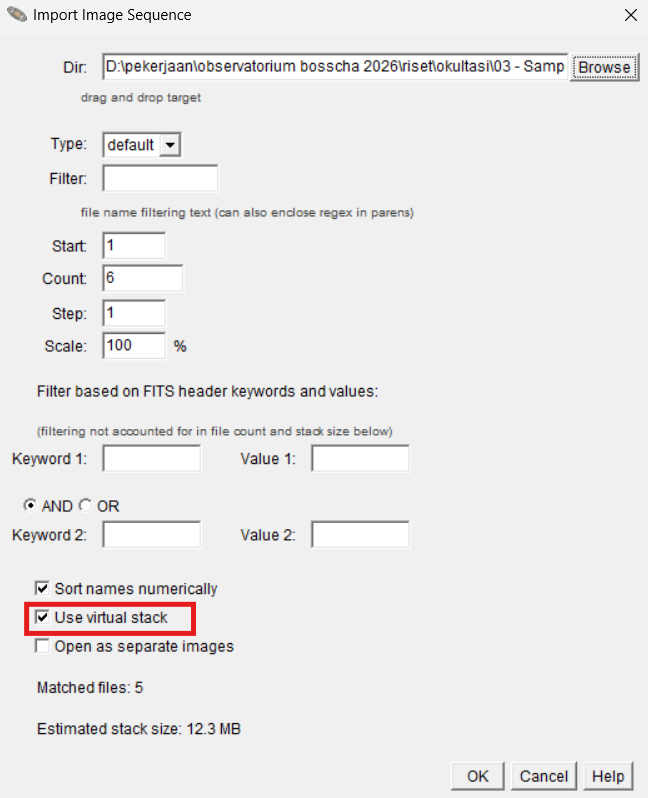
\includegraphics[width=0.5\linewidth]{snr_aij_virtualstack_update}
	\end{center}
	\begin{center}
		\includegraphics[width=0.6\linewidth]{snr_aij_toggle}
	\end{center}
	
	\item Tekan tombol alt + klik kiri pada bintang target, maka akan muncul profil seeing bintang tersebut. Catat nilai FWHM yang tertera pada judul gambar (pada contoh ini, FWHM = 6.77). Tekan tombol `Save Aperture' dan tutup jendela tersebut. Jika ada kesalahan menandai bintang, klik tombol \includegraphics[height=1em]{aij_clear} untuk menghapus aperture dan mengulangi. FWHM (\textit{Full Width at Half Maximum}) adalah ukuran yang digunakan untuk menggambarkan lebar dari profil cahaya bintang pada citra. Nilai FWHM ini akan digunakan untuk menentukan ukuran aperture dalam fotometri bukaan.
	\begin{center}
		\includegraphics[width=0.6\linewidth]{snr_aij_seeing}
	\end{center}
	
	\item Klik tombol \includegraphics[height=1em]{aij_set} dan ubah beberapa parameter berikut.
	\begin{center}
		\includegraphics[width=0.6\linewidth]{snr_aij_aphot_settings}
	\end{center}
	\begin{enumerate}
		\item Untuk kotak (1):
		\begin{itemize}
			\item \textbf{Radius of object aperture}: $\sim 1.5-2$ kali FWHM. Radius ini menentukan ukuran aperture yang digunakan untuk mengukur sinyal dari bintang target. Pastikan radius cukup besar untuk menangkap mayoritas sinyal, namun tidak terlalu besar sehingga memasukkan terlalu banyak noise latar belakang. Nilai $1.5-2$ kali FWHM adalah titik awal praktis; verifikasi kembali dengan kurva pertumbuhan (\textit{curve of growth}) pada data Anda.
			  
			  \underline{Contoh:} untuk FWHM = 6.77, maka radius yang direkomendasikan adalah sekitar $10-14$ piksel.
			\item \textbf{Inner radius}: tambahkan $\sim 3$ piksel dari \textbf{Radius of object aperture}. Hal ini untuk memberikan jarak aman dari profil cahaya bintang target dan memastikan area anulus latar belakang bersih dari kontaminasi bintang tetangga.
			\item \textbf{Outer radius}: tambahkan $\sim 5$ piksel dari \textbf{Inner radius}. Pastikan tidak ada bintang lain yang masuk dalam \textbf{Outer radius}.
			
			\underline{Catatan:} angka--angka di atas hanyalah \textit{guideline}. Cek dan sesuaikan dengan data yang dimiliki.
		\end{itemize}
		\item Untuk kotak (2):
		\begin{itemize}
			\item \textbf{CCD gain}: Nilai Gain adalah faktor konversi antara jumlah elektron yang diterima sensor dengan nilai digital yang tersimpan pada citra (ADU, \textit{Analog-to-Digital Unit}).
			Cek \textbf{CCD gain} untuk kamera Anda, biasanya tercantum pada spesifikasi kamera (terlampir adalah beberapa contoh kurva gain, sesuaikan dengan gain pada \textsc{SharpCap}). Jika data berasal dari ADC 12-bit yang diskalakan ke 16-bit, maka:
			\begin{equation}
				\mathrm{Gain_{input}} = \frac{\mathrm{Gain_{kurva}}}{16}
			\end{equation}
			sebaliknya jika diskalakan ke 8-bit, maka
			\begin{equation}
				\mathrm{Gain_{input}} = \mathrm{{Gain_{kurva}}}  \times {16}
			\end{equation}
			Jika kamera Anda memiliki ADC 16-bit, nilai gain yang dimasukkan adalah nilai gain dari kurva. 
			
			\underline{Contoh:} untuk ZWO ASI120MM--S pada gain 75 (nilai di \textsc{SharpCap}) dan data disimpan pada mode 16-bit dari ADC 12-bit, menurut kurva nilai gain--nya adalah $\sim 0.25$ $e^-$/ADU. Nilai yang dimasukkan pada kotak (2) adalah 0.25/16 = 0.015625 $e^-$/ADU.
			\begin{center}
				\includegraphics[width=0.7\linewidth]{snr_gain}
			\end{center}
			\item \textbf{CCD readout noise}: adalah noise yang muncul saat sinyal dari sensor dibaca dan dikonversi menjadi nilai digital (ADU). Noise ini berasal dari proses elektronik di dalam kamera, seperti penguat (amplifier) dan konverter analog-ke-digital (ADC). Silakan merujuk kepada kurva terlampir untuk kamera yang digunakan. Masukkan nilai dalam satuan $e^-$ rms/pixel pada gain yang sama dengan data Anda.
			
			\underline{Contoh:} pengamatan ini menggunakan gain 75, maka readout noise menurut kurva adalah $\sim 3.75$.
			\begin{center}
				\includegraphics[width=0.7\linewidth]{snr_readout}
			\end{center}

			\item \textbf{CCD dark current}: adalah noise yang dihasilkan oleh sensor kamera meskipun tidak ada cahaya yang masuk. Dark current disebabkan oleh elektron yang dihasilkan secara termal dalam sensor, dan nilainya biasanya meningkat dengan suhu. Pada kasus pengamatan okultasi, dimana waktu bukaan sangat pendek, nilai dark current biasanya sangat kecil dibandingkan dengan sinyal dari bintang target, terutama jika kamera dilengkapi dengan pendingin. Oleh karena itu, untuk perhitungan SNR awal, Anda dapat mengabaikan dark current.
		\end{itemize}
	\end{enumerate}
	Tekan OK untuk menutup jendela tersebut.
	
	\item Lakukan \textit{Star alignment}: klik \textit{Process > Align stack using WCS or apertures}.
	\begin{center}
		\includegraphics[width=0.6\linewidth]{snr_aij_align}
	\end{center}
	
	\item Pada jendela yang terbuka, pastikan \textit{First Slice} dan \textit{Last Slice} sudah sesuai dengan jumlah gambar (dalam contoh ini 5 gambar). Pastikan juga \textit{radius, inner radius, outer radius} sudah sesuai seperti poin sebelumnya. Sesuaikan \textit{setting} lain seperti pada gambar berikut. Tekan OK.
	\begin{center}
		\includegraphics[width=0.6\linewidth]{snr_aij_stackaligner}
	\end{center}
	
	\item Arahkan kursor pada bintang target dan klik 1x, maka akan muncul aperture berwarna hijau. Klik juga bintang--bintang lain yang cukup terang, maka aperture merah akan muncul. Setelah selesai, tekan `Enter'.
	\begin{center}
		\includegraphics[width=0.6\linewidth]{snr_aij_select}
	\end{center}
	
	\item Setelah \textit{alignment} selesai, tekan OK/Yes dan tutup jendela citra. Direktori baru bernama `aligned' akan muncul, berisi citra hasil \textit{alignment}. 
    
    \underline{Catatan:} Jika proses yang ada tidak menghasilkan direktori `aligned', ulangi langkah \textit{Import Image Sequence} dan pastikan `Use virtual stack' dicentang.
	
	\item Lakukan \textit{File > Import > Image Sequence} sekali lagi, namun arahkan ke direktori `aligned' dan tekan OK. Maka akan muncul kembali jendela file citra. Cek dengan tombol panah kanan dan kiri untuk memastikan semua \textit{frame} telah \textit{aligned}.
	
	\item Tekan tombol \includegraphics[height=1em]{aij_multiap} dan pastikan \textit{setting} kurang lebih seperti pada gambar berikut. \textit{First slice}, \textit{Last Slice} dan parameter \textit{radius} akan berbeda untuk setiap set data. Untuk memilih bintang pembanding secara manual, pastikan opsi `Auto comparison stars' tidak dicentang. Tekan tombol `Place Apertures'. 

    
	\begin{center}
		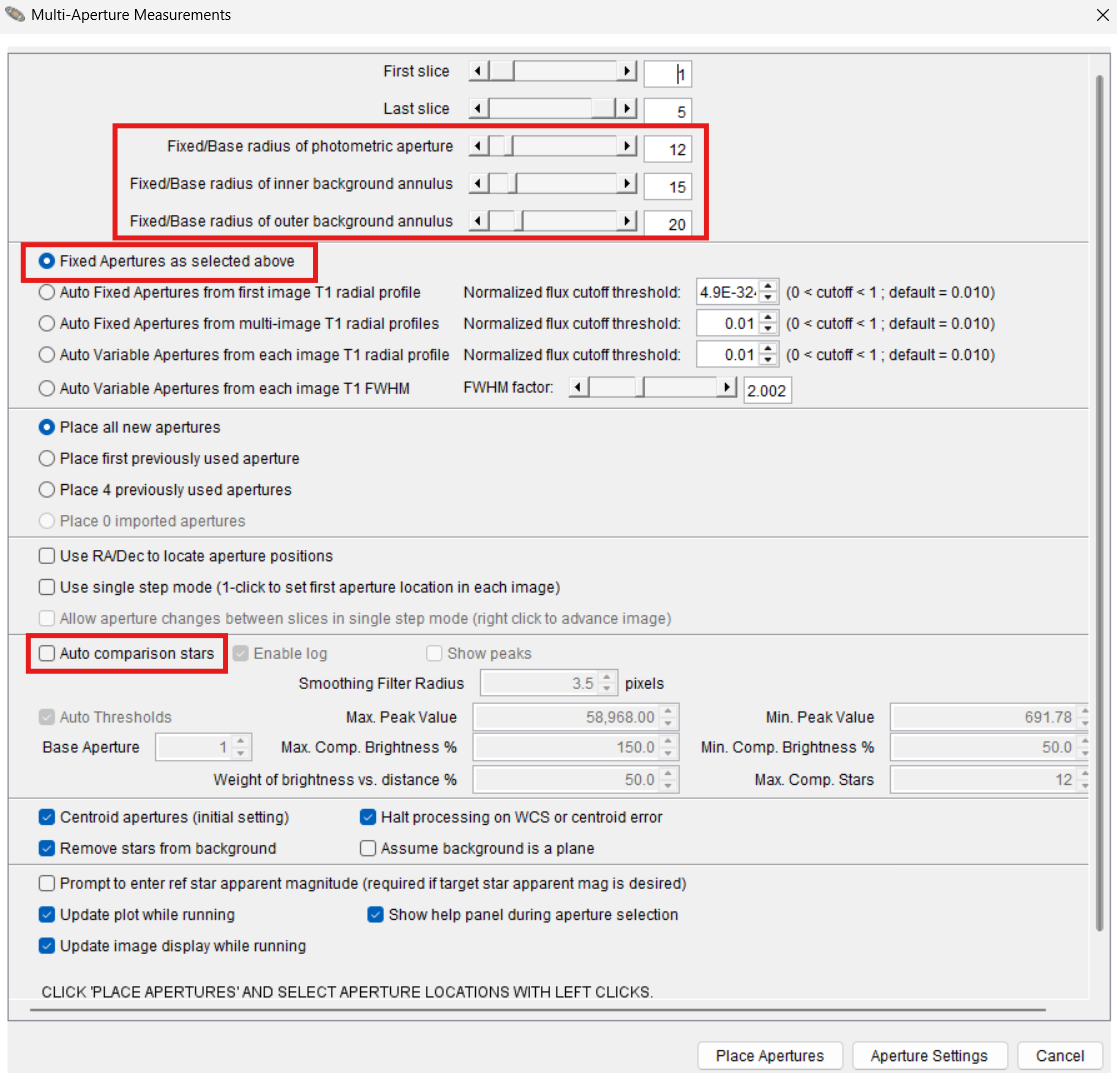
\includegraphics[width=0.6\linewidth]{snr_aij_multiap_measurement_update.png}
	\end{center}
	\begin{enumerate}
		\item Klik 1x pada bintang target (Pastikan bintang dipilih tidak salah. Jika salah, hapus dengan tombol \includegraphics[height=1em]{aij_clear}). Klik juga pada bintang lain sebagai pembanding (opsional, akan berguna jika Anda ingin melakukan fotometri diferensial). Sebagai contoh, pada dokumen ini, menggunakan 1 bintang pembanding (aperture merah). Tekan `Enter' untuk melakukan fotometri bukaan secara otomatis untuk semua frame. 
		\begin{center}
			\includegraphics[width=0.7\linewidth]{snr_aij_aphot}
		\end{center}
		
		\item Akan muncul banyak jendela, abaikan untuk sementara. Saat proses selesai, cari jendela `Measurements' (lihat gambar berikut) dan cari nilai SNR untuk target Anda (kolom Source\_SNR\_T1). Jika ingin mengetahui SNR untuk bintang pembanding, dalam kasus ini, Anda dapat melihat kolom Source\_SNR\_C2. Untuk ringkasan hasil, gunakan nilai median (atau \textit{sigma-clipped mean}) agar lebih tahan terhadap \textit{outlier}.
		\begin{center}
			\includegraphics[width=0.7\linewidth]{snr_aij_snr}
		\end{center}
	\end{enumerate}
	\item Selamat! Anda telah berhasil menghitung SNR data Anda.
\end{enumerate}
\end{document}